\section{Introduction}

While Magnetic Resonance Imaging (MRI) remains a promising source of biomarkers
for a variety of brain-related conditions, the reproducibility of MRI-derived
measures across analytical conditions has  been challenged in multiple contexts
over the past years. In structural MRI, cortical surface analyses have been
shown to be substantially affected by software, parcellation, and quality
control~\cite{bhagwat2021understanding}, in functional MRI, different research
teams analyzing the data have found only moderately consistent
results~\cite{botvinik2020variability}, and in diffusion MRI the variability
among white matter bundle segmentation protocols using diffusion MRI was found
to be comparable to variability across
subjects~\cite{schilling2021tractography}. The reliability of MRI-derived
measures critically depends on a better understanding and characterization of
the impacts of analytical variability, including
data selection, analytical decisions, tool selection, computational
infrastructure, and numerical
state~\cite{kennedy2019everything,kiar2024experimental}.

% Estimating variability
% is particularly important when effect sizes are moderate, as it is the case in
% studies of Parkinson's disease (PD)~\cite{he2020progressive}. 

Among these sources of analytical variability, numerical variability has been
shown to have a measurable impact on MRI
analyses~\cite{gronenschild2012effects,glatard2015reproducibility} but remains
understudied, mainly due to the practical challenges of quantifying its effects.
Numerical variability arises from rounding and truncation errors associated with
the use of limited-precision numerical formats, such as the widespread IEEE-754
standard for floating-point arithmetic~\cite{markstein2008new}. Numerical errors
manifest slightly differently across computational platforms (hardware,
operating systems, or library versions) and such differences sometimes
accumulate and amplify across computational analyses, eventually leading to
measurable differences in final
outputs~\cite{salari2021accurate,kiar2021numerical,des2023reproducibility,vila2024impact,chatelain2024numerical,mirhakimi2025numerical}.
Such issues occur particularly within high-dimensional optimization processes
such as linear and non-linear image registration, or the training of deep learning
models~\cite{gonzalez2025uncertain}.

The implications of numerical variability for clinical measures are unknown.
Previous studies focused on measuring its impact on image pre-processing   and
did not include any particular downstream analysis. The first aim of this study
was to quantify the impact of numerical variability in structural MRI analyses
of Parkinson's disease (PD), where robust MRI measures of the disease have yet
to be identified. We conducted typical cross-sectional and longitudinal analyses
of structural MRI data of PD participants, measuring numerical variability
through an experimental stochastic arithmetic approach.

Building on these observations, we developed an analytical framework and
associated tools to rapidly assess the numerical quality of structural MRI
analyses reported in the published literature, opening the possibility to
conduct large-scale impact evaluations of numerical variability. By making
numerical-variability evaluation accessible, our framework and tool enhance
transparency, support peer review, and promote more reliable statistical
inference in neuroimaging. Applying this framework to the PD literature, we
obtained the first estimates of the numerical quality of MRI analyses in
Parkinson's disease studies, highlighting a widespread impact of numerical
variability on MRI measures of PD.

\section{Results}

\subsection{Numerical variability alters statistical inference in MRI measures of PD}

We assessed the impact of numerical variability on conclusions
drawn from MRI analyses of Parkinson's disease, focusing on two common
analyses: (1) volumetric group differences between PD subjects and
Healthy Controls (HC), and (2) partial correlations between regional volumes and
motor evaluation scores measured with the MDS-Unified Parkinson's Disease
Rating Scale part 3 (UPDRS-III). For both, we conducted a cross-sectional
analysis at baseline and a longitudinal analysis across two time points.

We selected T1-weighted MRI data from the Parkinson Progression Marker
Initiative (PPMI) dataset~\cite{marek2011parkinson}, including participants with
at least two usable visits separated by 0.9-2.0 years, and excluding
participants with Mild Cognitive Impairment (MCI) or other neurological
disorders. The final dataset included  112 PD participants without MCI
(PD-non-MCI) and 89 HC participants (Table~\ref{tab:cohort_stat}).

We processed all images for both timepoints using FreeSurfer's
\texttt{recon-all}, introducing numerical noise via Monte Carlo Arithmetic
(MCA)~\cite{parker1997monte} to mimick realistic perturbations into this
pipeline. MCA injects random, zero-mean perturbations into floating-point
operations while perserving mathematical expectations. Such noise is
representative of the noise introduced by typical variations in hardware (e.g.,
CPU models), software libraries (e.g., operating system updates), or
parallelization (e.g., sequential vs multi-threaded executions). We repeated the
perturbed analyses, yielding 26 usable runs from which we estimated numerical
variability. We verified the validity of the numerical perturbation approach by
confirming that all unperturbed results belonged to the range defined by
numerically perturbed results.

For both group comparisons and correlation analyses, statistical outcomes varied
substantially across the 26 Monte Carlo Arithmetic (MCA) repetitions (Figures
\ref{fig:significance_correlation_subcortical_volume}
and~\ref{fig:significance_correlation_thickness}). For subcortical volumes (14
regions; Figure \ref{fig:significance_correlation_subcortical_volume}),
significance flipped in 27\% of of all (regions, analysis) pairs, indicating
frequent inconsistencies across repetitions. For cortical thickness (68 regions;
Figure \ref{fig:significance_correlation_thickness}), 21\% of (regions,
analysis) pairs were similarly unstable. These
fluctuations demonstrate that numerical noise alone can alter downstream
statistical inference in structural MRI analyses of PD.

\begin{figure}
    \includegraphics[width=\linewidth]{figures/consistency/subcortical_volume_significance_correlation.pdf}
    \caption{ Proportion of significant tests ($p<0.05$, uncorrected) for subcortical volumes
        across 26 numerical perturbations.
        \label{fig:significance_correlation_subcortical_volume}}
\end{figure}

\begin{figure}
    \centering
    \includegraphics[width=\linewidth]{figures/consistency/cortical_thickness_significance_correlation.pdf}
    \caption{Proportion of significant tests ($p<0.05$, uncorrected) for cortical thickness
        across 26 numerical perturbations.\label{fig:significance_correlation_thickness}}
    \label{fig:navr_consistency_thickness_plot}
\end{figure}


\subsection{A practical model to quantify the impact of numerical variability}
% Comments:
% - Build a tool that can be broadly applied to any neuroimaging
% - Analytical modeling of sigma_d
% - Explain why having a tool is important
% - Why having a tool fast is important
%   - Measuring numerical variability is a time-consuming process
%   - Analytical modeling of sigma_d allows applying the tool to any
%     neuroimaging papers, existing results.
% - Quality Control impact findings => a tool to find potentially unreliable
%   results
% - To be general, we developped an analytical model
% - Refers to the online tool on yohanchatelain.github.io/brain-render

% \TG[done]{Instead of re-stating the importance of numerical variability in this
%     paragraph, which supposedly should be understood from the end of the
%     introduction, here you could explain the need for a tool to quickly and
%     practically evaluate its impact in a given study, explain and justify your
%     assumptions (e.g., numerical variability is a feature of the pipeline rather
%     than the population---refer to previous works). In doing so, you could explain
%     how running MCA is currently not realistic due to computational requirements
%     (although new architectures may enable it in the coming years), and explain the
%     need for a statistical correction.}

While the previous results demonstrate that numerical variability can alter
statistical inference in MRI analyses of PD, routinely conducting computationally
expensive Monte Carlo evaluations is impractical for most studies. To address
this issue, we developed a closed-form analytical model that predicts numerical
uncertainty using only standard summary statistics. The core of this framework
is the Numerical-Population Variability Ratio (\navr), defined as the ratio
between numerical variability ($\sigma_{\mathrm{num}}$; Eq.~\ref{eq:sigma_num})
and population variability ($\sigma_{\mathrm{pop}}$; Eq.~\ref{eq:sigma_anat}):
\[
    \nu_{\mathrm{npv}} = \frac{\sigma_{\mathrm{num}}}{\sigma_{\mathrm{pop}}}
\]

The \navr metric standardizes the quantification of numerical instability,
enabling direct comparisons across different brain regions, software pipelines,
and cohorts. By propagating this ratio through standard statistical estimators
using the delta-method (see Section~\ref{sec:theoretical_derivations}), we
derived approximations for the numerical uncertainty in common
statistics (Table~\ref{tab:stat_uncertainty}) and validated them through
numerical simulations. This framework establishes a direct link between a
pipeline's numerical instability (\navr), the study's sample size ($n$), and the
resulting reliability of p-values and effect sizes. Crucially, because these
formulas rely solely on summary statistics, they allow for the retrospective
quality control of existing literature without requiring access to original raw
data or costly re-computation.

% \TG[done]{I think I would rather present the $\sigma_d$ result first, then explain
%     NAV. When introducing sigma d, you could better explain that numerical
%     variability has to be evaluated in the context of a particular effect size, and its impact will be dependent on sample size.}

\begin{table}[ht]
    \centering
    \begin{tabular}{lll}
        \toprule
        \textbf{Statistic}
                            & \textbf{Numerical standard deviation}
                            & \textbf{Numerical p-value uncertainty}                                                                                                           \\
        \midrule
        Cohen's $d$         & $\sigma_d \approx\nu_{\mathrm{npv}}\frac{2}{\sqrt{n}}$             & \multicolumn{1}{c}{-}                                                       \\
        Two-sample $t$      & $\sigma_t \approx \nu_{\mathrm{npv}}        $                      & $\sigma_{p} \approx 2f_{t,df}(|t|)\nu_{\mathrm{npv}}$                       \\
        Partial correlation & $\sigma_r \geq \nu_{\mathrm{npv}}\sqrt{\frac{(1-r^{2})^{3}}{n-1}}$ & $\sigma_{p} \geq 2f_{t,df}(|t|)\sqrt{\frac{df}{n-1}}\nu_{\mathrm{npv}}$     \\
        ANCOVA              & $\sigma_F \approx 2\sqrt{F}\nu_{\mathrm{npv}}$                     & $\sigma_{p} \approx 2\sqrt{F}f_{\mathcal{F}}(F;1,df_2)\,\nu_{\mathrm{npv}}$ \\
        \bottomrule
    \end{tabular}
    \caption{First-order numerical uncertainty of common statistical tests under
        Monte Carlo Arithmetic perturbations. Cohen's d formula assumes large
        and equal group sizes. $f_{t,df}$ and $f_\mathcal{F}(F;1,df_2)$ denote
        the probability density functions of the Student's $t$-distribution with
        $df$ degrees of freedom and the $\mathcal{F}$-distribution with $(1,
            df_2)$ degrees of freedom, respectively. The $p$-value approximation for
        the partial correlation uses $t=r(df/(1-r^2))^{1/2}$.}
    \label{tab:stat_uncertainty}
\end{table}

We applied this model to quantify the stability of the analyses reported above
(Figure~\ref{fig:navr}). In cross-sectional baseline analyses, the average \navr
was 0.191 for the PD group and 0.176 for HC, with no significant difference
between groups (permutation test, $p > 0.05$; Appendix
Figure~\ref{tab:bootstrap-navr}). Applying the Cohen's $d$ uncertainty formula
(Table~\ref{tab:stat_uncertainty}) to these \navr values reveals that
suppressing numerical uncertainty to a negligible level ($\sigma_d \leq 0.01$)
in cross-sectional studies would require approximately 1,340 participants.

In contrast, longitudinal analyses exhibited substantially higher instability,
with average \navr values of 0.561 for PD and 0.549 for HC although no
significant difference was found between groups (permutation test, $p > 0.05$;
Appendix Figure~\ref{tab:bootstrap-navr}). This amplification is
likely driven by catastrophic cancellation that occurs when subtracting nearly
identical values between timepoints.  Consequently, achieving the same level of
numerical uncertainty ($\sigma_d \leq 0.01$) would require a sample size
exceeding 12,000 participants, highlighting the critical impact of numerical
noise on reliability.

To facilitate the use of this framework, we developed an
open-source, interactive web interface available at
\href{https://yohanchatelain.github.io/brain\_render/}{yohanchatelain.github.io/brain\_render}
(Appendix Figure~\ref{fig:brain_render_tool}). This tool allows researchers to
upload standard summary statistics to instantly estimate the numerical
uncertainty floor of their findings. The interface
includes a 3D visualization engine that maps uncertainty onto cortical and
subcortical atlases, allowing for interactive exploration of pipeline stability.
To aid interpretation, the tool automatically flags regions where the reported
effect size is indistinguishable from the estimated numerical noise,
thereby identifying potentially spurious findings.

\begin{figure}[h]
    \centering
    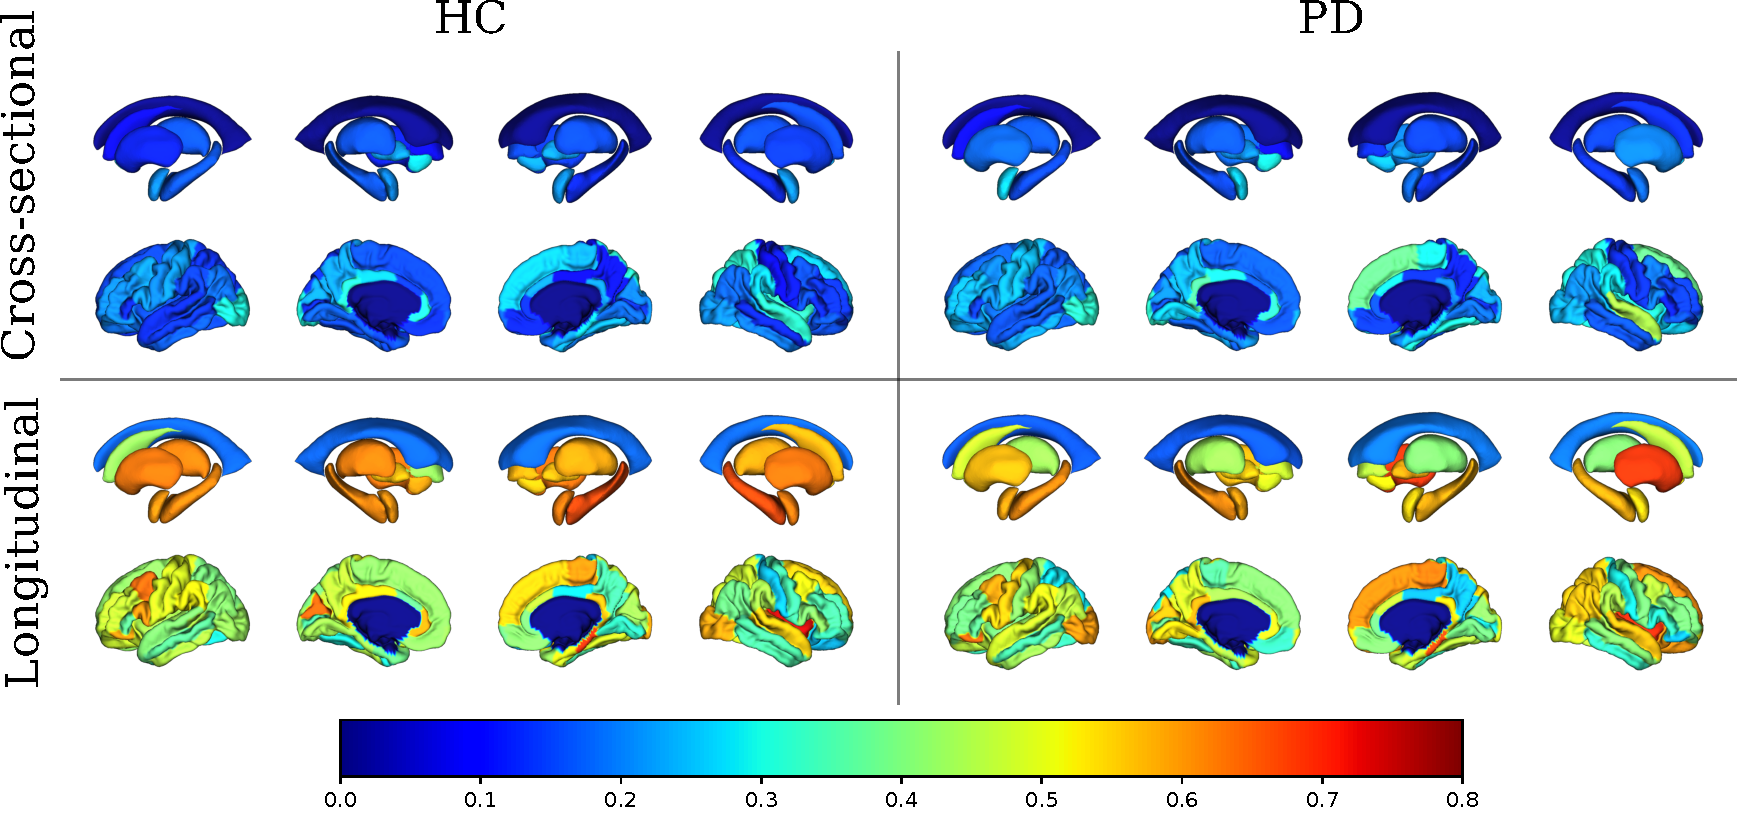
\includegraphics[width=\linewidth]{figures/NPV_map/figure_3.pdf}
    \caption{Numerical-Population Variability Ratio (\navr) for subcortical
        volumes (top row in each panel) and cortical thickness (bottom row in
        each panel) in healthy controls (HC) and Parkinson's disease (PD).
        Higher \navr values indicate higher computational
        uncertainty relative to inter-subject variability.}
    \label{fig:navr}
\end{figure}

% \begin{figure}
%     \includegraphics[width=\linewidth]{figures/sigma_d_contour.pdf}
%     \caption{\TG{could you show some of the papers in this figure? } Relationship between \navr and population sample size  \(N\) for
%         predicting the uncertainty in Cohen's d effect size estimation. The
%         contour lines represent different \navr values, showing how numerical
%         variability scales with sample size. With a typical \navr value of 0.2,
%         to maintain reliable effect size estimates $\sigma_d \leq 0.01$, the
%         plot suggests to use $N \geq 1500$.\label{fig:sigma_d_contour}}
% \end{figure}

\subsection{Impact of numerical variability on published findings}

To assess the broader implications of numerical variability on MRI measures of
Parkinson's disease, we applied numerical uncertainty propagation
(Table~\ref{tab:stat_uncertainty}) to re-evaluate findings from thirteen articles
reporting MRI measures of Parkinson's disease,
namely~\cite{chagas2017neuroimaging,garcia2014structural,gerrits2016cortical,
    hanganu2014mild,lewis2016pattern,li2022cortical,mak2014subcortical,
    pellicano2015morphometric,radziunas2018brain,sokolowski2024impact,
    sokolowski2024longitudinal,wilson2019cortical,yang2024longitudinal}.
These studies were selected to illustrate the potential impact of numerical
variability on reported outcomes based on available summary statistics.

For each p-value reported as significant in the original articles, we calculated
the associated numerical uncertainty using the formulas in
Table~\ref{tab:stat_uncertainty}. We then estimated the probability of a
significance flip where a result transitions from significant to non-significant
due to numerical error by modeling the true p-value as a Beta distribution. We
parametrized this distribution such that the reported p-value represents the
mean and the calculated numerical uncertainty represents the standard deviation.
By computing the cumulative distribution function of this characterized Beta
distribution at the original significance threshold, we derived the probability
that the reported significant finding was, in fact, a numerically induced false
positive.

Figure~\ref{fig:false_positive_vs_sample_size} displays the probability of such
false positives as a function of the sample size, across different statistics.
The thirteen articles in the figure have been anonymized as our goal was not to
single out particular results. Substantial probabilities of numerically-induced
false positives were observed, across sample size, statistics, and analysis
types. These results indicate a widespread impact of numerical variability on
MRI measures of Parkinson's disease, highlighting the need for more systematic
numerical evaluations in MRI studies.

% \TG{I have reworded the previous paragraph (still available in Latex comments)
%     as your four claims would need to be backed by statistical tests, which I don't
%     think makes a lot of sense given the scarcity of the data.}
% Our analysis yields four key observations. First, no specific statistical test
% appears inherently more robust to numerical variability than others. Second,
% contrary to standard statistical intuition regarding sampling error, sample
% size does not appear to mitigate the probability of numerically induced false
% positives; for example, cross-sectional volume analyses exhibited similar
% instability magnitudes at sample sizes of both 43 and 315. Third, while
% longitudinal analyses generally showed lower false positive probabilities than
% cross-sectional analyses, they simultaneously exhibited higher \navr. This
% apparent contradiction suggests that the proximity of a p-value to the
% significance threshold is the primary driver of instability: p-values hovering
% near the threshold are highly sensitive to numerical noise, regardless of the
% study design. Finally, cortical measures demonstrated higher false positive
% probabilities compared to subcortical measures, indicating a greater
% sensitivity to numerical variability in cortical measures.

\begin{figure}
    \includegraphics[width=\linewidth]{figures/figure-distance-paper.pdf}
    \caption{Probability of numerically-induced misclassifications in function
        of p-value distance to significance threshold across different
        statistics: T-values (T), F-values (F), and correlation coefficients
        (R). The marker's size reflects the sample size.
        \label{fig:false_positive_vs_sample_size}}
\end{figure}


\section{Discussion}

% Comments:
% 1. Summarize the main results and what do they mean
% 2. Extension beyond FreeSurfer and expectation to generalize the findings to other neuroimaging software
% 3. Discuss the potential sources of numerical variability (minimal local, minimal precision, etc.)

% [] Mention using neuroimaging as biomarker (n=1 scenario), personalized medicine,

In this study, we demonstrate that numerical variability arising from
floating-point computation constitutes a substantial source of variability in
structural MRI analyses of Parkinson's disease, accounting for up to 93\% of
population variability \TG{check value, can we report the average
    $\nu_{nav}$ observed in PD participants?}. By systematically perturbing the FreeSurfer pipeline
using Monte Carlo Arithmetic, we show that numerical noise alone can account for
a non-negligible fraction of population variability in both cortical and
subcortical measures. This variability is sufficient to alter downstream
statistical inference, leading to frequent significance flips in group
comparisons and clinical correlations, even when a pipeline configuration and
computational environments are held constant. These findings provide a concrete
computational mechanism that helps explain persistent reproducibility challenges
reported across clinical neuroimaging.

The Numerical-Population Variability Ratio (NPVR) introduced in this work
formalizes numerical variability as a quantity directly comparable to population
variability. By analytically propagating NPVR through common statistical
estimators, we establish explicit relationships between computational
instability, sample size, and uncertainty in effect sizes and p-values. This
framework shows that numerical uncertainty does not vanish with increasing
sample size in the same manner as sampling error, and that results near
conventional significance thresholds are sensitive to numerical perturbations.
Crucially, while applied here to numerical instability, this formalism is
generalizable: the NPVR could model the propagation of other independent error
sources, such as test-retest variability or instrumentation noise, offering a
unified perspective on non-sampling errors.

Importantly, NPVR enables practical numerical quality evaluation without
requiring access to raw imaging data or expensive re-processing. Applying this
framework to previously published Parkinson's disease MRI studies revealed that
a fraction of reported significant findings are susceptible to numerically
induced instability. These results underscore that numerical variability is not
a technical artifact but a factor that can directly influence scientific
conclusions. By making this assessment feasible from summary statistics alone,
NPVR offers a scalable approach for retrospective evaluation of the numerical
robustness of the existing literature and prospective evaluation of new studies.
\TG{can we make recommendations for people to evaluate false positive rates
    using your tool or any other simple mean?}

Although our empirical analyses focused on FreeSurfer 7.3.1, the observed
instabilities are not unique to this software. Prior
work~\cite{mirhakimi2025numerical}~\YC{cite Mathieu} has documented comparable
numerical sensitivity in other widely used neuroimaging pipelines, including
FMRIB Software Library~\cite{jenkinson2012fsl} (FSL) and Advanced Normalization
Tools~\cite{avants2009advanced} (ANTs), while suggesting lower sensitivity in
Statistical Parametric Mapping~\cite{ashburner2009computational} (SPM),
potentially due to differences in optimization strategies and regularization.
These findings indicate that numerical variability is a property of
computational pipelines rather than a specific implementation artifact. The
magnitude of the uncertainty then depends on algorithmic design choices,
numerical precision, and optimization dynamics.

The increasing adoption of deep learning-based components in neuroimaging
pipelines does not eliminate numerical variability but instead shifts its focus.
The latest FreeSurfer release (v8) now integrates deep learning models such as
FastSurfer~\cite{henschel2020fastsurfer} and
Synthmorph~\cite{hoffmann2021synthmorph} to replace classical segmentation and
registration steps. While inference in trained models can be relatively
stable~\cite{pepe2023numerical}, training itself introduces additional sources
of variability, including stochastic optimization, weight initialization, and
floating-point precision effects. Recent work~\cite{gonzalez2025uncertain}
suggests that these factors can lead to different trained models under identical
initial conditions, echoing the sensitivity to local minima observed in
classical nonlinear optimization. Quantifying and controlling numerical
variability across both classical and learning-based approaches remains
therefore a critical challenge for the field.

We considered several factors that may influence the generalizability of our
findings. The Parkinson's disease cohort analyzed here is relatively homogeneous
in age and phenotype, which could reduce population variance and inflate NPVR
estimates. However, we observed no significant differences in numerical
variability between patients and healthy controls, supporting the interpretation
that numerical instability is primarily a property of the computational pipeline
rather than the clinical population. Extending NPVR measurements across diverse
datasets, disease contexts, and software packages will be important to build a
comprehensive map of computational reliability in neuroimaging, though our
results already suggest that numerical variability is sufficiently large to
warrant routine consideration.

More broadly, this work highlights that computational uncertainty should be
treated as a serious component of uncertainty in neuroimaging, alongside
biological variability and statistical sampling error. Floating-point rounding
and truncation are only one contributor; algorithmic choices, preprocessing
decisions, and data handling practices all interact with numerical precision to
shape final results. Extending this quantification to the deep-learning training
stage is equally important, given the field's central role in modern
neuroimaging, and would support more robust and interpretable models. Systematic
quantification of these effects is essential for the development of numerically
robust software and for the reliable translation of neuroimaging biomarkers into
clinical and personalized-medicine settings.

In conclusion, NPVR provides a principled, interpretable, and scalable framework
to expose hidden numerical instability in neuroimaging analyses. By enabling
routine evaluation of numerical uncertainty, this approach strengthens
transparency, supports more reliable inference, and offers a concrete path
toward improving reproducibility in computational neuroscience.
